%%
%%  Department of Electrical, Electronic and Computer Engineering.
%%  EPR400/2 Final Report - Section 1.
%%  Copyright (C) 2011-2018 University of Pretoria.
%%

\section{Literature Study}

Two core designs are to be integrated for the successful development of the home shopping list device. These designs are the design for handwriting processing and device to device communication. The research done on the theory associated with these designs is discussed in this section.

Handwriting processing can be subdivided into handwriting recognition which is applied from the pre-processing to the processing stages and handwriting analysis, which is mainly applied in the post-processing stage. For handwriting recognition, the goal is to convert grey scale images of handwritten text into machine-recognizable code at an acceptable level accuracy. The user will write their shopping list data on the device’s touchscreen and the device must convert this handwritten data into ASCII text. The device’s handwriting recognition scheme can either be offline or online handwriting recognition. The different models from either of these schemes can be classified as either bottom-up or top-down models.

Bottom-up models involve the analysis of neuro-centric processes at the lowest level of abstraction. The processes analysed are those involved in the simplest input of a character to the full input of a handwritten word. Top-down models are most applicable to this project because they are familiar with language processing tasks like speech recognition. The models that are categorized as top-down can be sub-divided into discrete and oscillatory models. 

In discrete models, handwritten pen inputs are defined as the vector sum of the discontinuous pen strokes. On the other hand, oscillatory models classify oscillations as simple pen movements on the input surface therefore handwritten inputs are defined as suddenly interrupted pen movements.

In online handwriting recognition, a user inputs their data using a touch pen or any other stylus that provides a distinct pattern on the input surface e.g. ink. The stylus’s successive trajectories are recorded as vectors with x and y co-ordinates. This means the user’s order of inputting their characters is recorded in a 2-dimensional array. The recognition algorithm is then applied to these vectors and the input data is converted to ASCII text on the go. Therefore, the user gets real time feedback from the recognition scheme [2]. No recognition scheme can work perfectly so the advantage of this scheme is that incorrect conversions or errors can be corrected almost instantly. A timer is used so that after a certain period, when the pen is lifted or there is no input the array is saved. The recognition algorithm is applied to this array and the next time the stylus inputs another handwritten character, the saved already saved character has already been converted to the equivalent ASCII text and the array cleared. The next handwritten character’s co-ordinates are pushed into this empty array. If recognition is not finished, then another array is used. The arrays for saving the handwriting input therefore follow a queue format [6]. Queuing models are represented by Kendall’s notation. The typical Kendall’s notation is shown in the equation below.

\begin{equation}
	\text{Queue} = A/S/k
\end{equation}

In the equation, A represents the arrival rate. In the online handwriting recognition case, this is the rate that the vector arrays are saved. Since the time that a user finishes their input cannot be predicted and varies for each input sequence, it can be assumed to be non-deterministic and the cumulative time that the co-ordinates are saved can be assumed to follow an exponential series which can be modelled by a Poisson distribution. S represents the service rate. In the online case, this is the rate at which the saved arrays are converted to their equivalent ASCII text. This is non-deterministic as well and can be assumed to follow an exponential rate. This is due to the fact that the recognition rate has direct dependence on the sequence of co-ordinates in the array and these are non-deterministic. k represents the number of servers in the queuing system.  In this case the servers are modelled by the character recognition algorithm converting the 2-dimensional array into the equivalent ASCII code and clearing the array thereby freeing memory. This algorithm only operates on a single 2-dimensional array of the co-ordinates at a paticular time. No handwriting conversions can occur concurrently therefore the number of servers in the queuing system is equal to 1. The queuing system involved in the waiting for the array to be cleared can therefore represented by the model below:\\
\begin{equation}
	\text{Queuing model} = M/M/1
\end{equation}

Where:

\hspace{10mm} M = Markovian distribution which represents the arrival rate.

\hspace{10mm} M = Markovian distribution which represents the service rate.

\hspace{10mm} 1 = Number of servers.

Using the queuing model properties from [3], the average number of arrays used in the handwriting recognition process can be calculated. This leads to an easier calculation of the average amount of memory used in the online handwriting recognition process. This is calculated to be in the “Byte-range” in the worst case. This means this process is extremely memory-efficient since even the simplest everyday devices with micro-chips have millions of Bytes in memory at worst.

Online handwriting recognition is mainly focussed on three domains; digital signatures, pen-input devices and developmental tools. Digital signatures domain involves the use of well-trained recognition algorithms to verify a user’s identity to access important features e.g. bank account transactions. Pen-based device domain involves pen-input computer platforms recognizing handwriting or gestures from a user through a pen. Developmental tool domain involves the use of integrations of systems that take advantage of the neuro-centric property of handwriting recognition to develop and implement education and disability-assisting systems e.g. speech recognition algorithms to recognize and change voice to text for easier communication with the hearing-impaired. Our end goal is to develop a device that accepts touchscreen inputs and converts that to text. Therefore, this will fall in the pen-based devices domain. The domain is expanded to process electronic ink in the form of the pen’s drawing on the touchscreen.

Before the execution of the recognition phase, the handwritten input goes through a pre-processing phase. In this phase, noise is filtered from the input. Next, the skew within the pen input is corrected or normalized. The final stage of this phase involves the segmentation of the pen input into separate meaningful characters. Some models like Markovian models skip over this part to recognize the whole word that is input by the pen using probabilistic means which do not require segmentation. Therefore, segmentation is involved for models in which machine learning is involved.
There are various sources of noise for the handwriting input. The most common source is the user’s finger or hand randomly making contact with the touchscreen when the user intends to write using the pen. The capacitive touchscreen has no way of differentiating the pen from the fingers, so those motions are recorded as handwriting input. Another source of noise could be the pen used. Most of the pens used for touchscreens contain rubbers at their tips. The material used for the rubber directly affects the handwriting input. If the material is too large, then noise is introduced to the input by appending unwanted features to the drawn characters or words. However, the tip has to be large enough for the drawn input to be recognizable, so a trade-off is made for the right type of pen to have a significant size for its tip as long as the noise it produces is filterable or small enough to be differentiable from the actual input. Another source of noise is the touchscreen’s drawing application introducing a certain amount of quantization noise. Noise can be removed from the handwriting input by digital processing methods like signal filtering and data smoothing [5].

Skew normalization is normally applied to recognition systems which accept cursive word input. In this case, the slant on the skewed word is checked against a certain limit that is pre-defined e.g. a maximum of 45o to the right. Therefore, the required skew adjustment angle will be calculated by finding the difference between the skew angle and limit e.g. 45o in this example case. If the skew angle is less than the limit, then no skew correction is necessary.
\begin{equation}
	skew_{correction} = skew - limit
\end{equation}

The skew above the limit is compensated for by shifting the cursive by the value of $skew_{correction}$. 

Segmentation applies at two levels. In the first, it is involved in the separation of equations, lines contained in a paragraph into different lines and the words in a specific line into different words. At this level, spatial zones [6] are defined so that trivial units are extracted from a paragraph. This level works for inputs which are provided in a paragraph format. It could also work in the practical case for line inputs by separating the line into different words of shopping list items. In the 2nd level associated with segmentation, input is separated into individual characters. This is lowest level of segmentation of importance. Therefore, after the paragraphs are segmented into separate lines and lines are segmented into different words, the different words contained in each line are separated into individual characters. This is hardest part of the pre-processing phase because it involves the separation of cursive words into individual characters. Separating cursive words means determining where each character starts and ends. The obvious risk is that a character’s features can be incomplete and be appended to the next character’s features leading to a character that is incomplete and another that is unknown. This error carries over to the recognition process where the probability of recognizing both these characters correctly is reduced. Most segmentation is carried immediately before the recognition process by using machine learning, namely convolution neural networks to separate the cursive text into characters.

The recognition process can be split into two classes, rule-based methods and structural methods. Structural methods involve the abstract definition of character shapes [7]. The shape variations involved in the practical real-world applications of the recognition process are ignored. Rule-based methods involve the use of flexible rules that use statistical models to determine frequency of occurrence of certain features [8] in a shape. The statistical models associated with these methods can either be explicit, implicit or Markovian. Explicit statistical models generally follow linear distributions, but they require a lot of memory and processing speed. Implicit models involve the use of natural networks for the training of pen input and learning from predefined test results. Error correction is done by using by using back-propagation in the neural network and the future handwriting input learns from the already tested dataset. Markovian models involve an under-the-surface process whereby state changes occur depending on the conditional probabilities associated with each state. Markovian models can be used as a work-around segmentation when dealing with cursive word input.

On the other hand, when offline handwriting recognition is used, the whole document is scanned. This scanned document is converted to an image and the recognition algorithm is applied to the whole image so that the whole paragraph is converted to the equivalent ASCII text. An interrupt can be programmed so that scanning is done periodically. The user only gets feedback from the scheme after the whole document has been scanned and converted to text.

The same pre-processing steps applied in online handwriting are usually applied to offline handwriting. The image taken from the scanner must be converted from grey-scale to binary in the step called thresholding. In the binary converted image, the scanned input will now be in black and white. The binary values of 1 and 0 are assigned to the two colours. The image is different into any pixels and each pixel is represent by a bit. A bound is pre-set to define the border between a pixel which is black and one which is white. The bits representing the pixels are then added to a 2-dimensional array. The rows of the array contain the pixels of the image in the width spectrum while the columns represent the image pixels in the height spectrum. It is important to note that this array is the one that is the argument of the recognition algorithm after the segmentation and other noise removal processes. 

Since digital capture is the most popular image capturing technique in offline recognition, noise is inherently most likely to occur from the device used to scan the images. These disturbances can be rectified using a smoothing process. Another popular problem associated with offline recognition is the overlap of successive lines in a paragraph due to skewing. A possible solution is the use of thinned images to follow the scanned strokes linearly and segment the interfering strokes from the signal. Instead of removing this signal, it’s coordinates, and shape are noted and appended to the next thinned line which will be missing this information. This correction may require skew correction on the part of the segmented strokes. 

For many skewed scanned images, the approximate skew angle is similar globally. An example is shown in the image that follows.\\
\newpage
\begin{figure}[h]
	\centering
	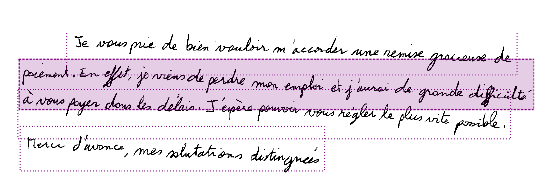
\includegraphics[scale=0.9]{1}
	\caption{An example showing global skew in a scanned image}
\end{figure}
\nocite{Haykin:Communication_Systems}
The scanned handwritten paragraphs have to be segmented into lines, then into words and finally into characters. The task of line segmentation is complex since handwritten text is normally written into non-symmetrical imaginary lines and these lines overlap up and down as shown in Figure 2, thus affecting neighbouring lines’ line input. The most popular method is estimating global angles of both vertical and horizontal skew. These angles are normalized as is done in online recognition skew correction. The space is repeated from the assumed initial line of the image to the last line. The local minimum of each captured line is approximated to be the baseline [104] for each line and these minima are concatenated to classify all the lines. For word segmentation, each segmented line is then split into its constituent words. The most popular scheme is using a rule-based approach where physical gaps are defined and if the gap size or higher is encountered, then a preceding word is separated from the next one. The assumption in using this approach is that the space between consecutive words is assumed to be bigger than the space between consecutive characters in a word. After separating the line into words these words have to be converted to ASCII text. These words are either passed to the recognition algorithm or they are further segmented into different characters. Word-level recognition uses statistical models which are discussed later. Most of the recognition schemes require character input so the words need to be further split into characters. Special features like concavities [102] are incorporated to determine segmentation points. The segmentation algorithm incorporates rules that compare gaps between segments to obtain the different characters.

A major difference between the pre-processing steps of offline and online handwriting recognition is that character segmentation in offline recognition is normally associated with non-cursive text while online recognition normally deals with cursive handwriting input.

The word-recognition algorithm is used, and the word image is compared to options in a lexicon and a list of the most probable words is returned. The recognition approach can either be holistic or analytic. When a holistic approach is used, the whole word image is immediately converted to equivalent ASCII text normally by statistically based models. On the other hand, an analytical approach recognizes the segmented characters of the word and then combines the results at the end.

Comparison between the two handwriting schemes shows that it is easier to correct conversion mistakes when using online handwriting recognition since feedback is provided after each character input. In contrast, since a whole document is scanned in offline recognition there will be multiple mistakes observed after each conversion and correcting these errors is a lot of work compared to when using online handwriting recognition. This is because conversion in offline recognition is on a paragraph level, which means in the worst case, there will most likely be errors for every word, in every line in every paragraph. In comparison, the worst case in online handwriting is an error in recognizing the preceding character which is far easier to fix by just rewriting the character.

Most handwriting recognition schemes have their accuracy dependent on how close the user’s handwriting is to the standard training sets, which are the IAM and the MNIST data set. The home shopping list device to be developed adds onto the already used datasets so that multiple user handwriting styles can be converted to ASCII text at an acceptable accuracy level, which is 80$\%$ or more in this case as shown in the project proposal section.

A hybrid of the two recognition schemes will be used in this project. Shopping list data will be input onto the touchscreen line by line. A touch pen will be used to input each line, as is done in online recognition and after each line the user will click a button to convert the line. After this button is clicked, the user input on the touchscreen will be converted to an image, as is done in offline handwriting recognition. The recognition algorithm will then be applied to convert this image into a line of text. This method makes use of the best traits of both online and offline handwriting recognition. Recognition is done on a word level, meaning a dictionary can be used to disregard character recognition errors. This dictionary contains a list of pre-defined words, in this case words that are normally found in a large-scale grocery store. 

The methods that have been developed to solve this problem are statistical models like Hidden Markov Models and machine learning models like neural networks. Hidden Markov models involve the use of probability distributions to calculate the chances of state transitions which relate to the probabilities of certain words being next to each other for character recognition. An algorithm called the Viterbi algorithm is then used to connect and detect the most likely sequence detected, which is not necessarily the most likely characters detected but the most likely word handwritten. On the other hand, neural networks work mostly with individual character recognition, with the emphasis being on training the network enough so that it can correctly detect unseen handwritten data passed to it. It is clear that the best scheme is somewhere in the middle of the two schemes analyzed so the best way could be integrating them and taking the best features provided by each scheme. 

The device to device communication design is useful for communication between the shopping list device and the user’s mobile phone. The various communication techniques available are grouped into either wireless or wired communication. The user will need to send a text-file containing their shopping list from the shopping list device to their mobile phone.  

Wired communication involves the direct use of cables and wiring for the transfer of data. The most popular application of wired communication is the use of a telephone. The telephone is connected directly to the local telephone switch using wires from the user’s home to the local telephone switch station [48]. The wires used could either be copper wires or optical fibres. Most modern wired systems use optical fibres because they are capable of carrying more signals compared to the traditional copper wires. Telephone service providers usually provide internet access with the same wiring using used for basic telephone communication. A splitter can be used to allow a single incoming wired connection to provide both internet access as well as the basic audio network for making and receiving calls. Wired connections are the most stable and are not easily affected by weather. When a wired connection is used instead of a wireless communication the signal strength will be higher and the transmission speed will be faster. 

The most popular type of wire used is the twisted pair wire. This type of copper wire is used for both the transmission of data as well as basic telephone communication. This wire achieves one of the fastest data transmission rates possible i.e. 100 Mbps. Although the wire is cheap, it can only cover a maximum distance of 100 m which is way below the desired transmission distance which is limitless. Another type of wire used in wired communication is a coaxial cable. The cable contains a copper wire at the centre surrounded by insulation tape. Transmission speeds can reach up to 10 Mbps and it is mainly used in television broadcast transmission as well as broadband communication. The fastest growing cable used in wired connections is the fibre optic cable. The most important property of these cables is that each cable contains thin plastic strings that carry data by reflecting light. The strings can be made of glass to increase the cable’s reflecting capability. These cables can transfer data at speeds of up to and greater than 10 Gbps.

The use of wires in this communication scheme means that the connections are susceptible to corruption by physical means [49]. Some of these data corruption mechanisms include attenuation. Data transmission can also be delayed due to earthquakes or other natural disasters that may affect the wires for the connection. Since copper wires have to be used for long distances where homes can be up to 30 km from the central station, they cannot be under surveillance for all this distance in remote areas and are thus susceptible to theft. Wired communication is most adequate for real-time high-bandwidth requiring operations like live video streaming.

On the other hand, wireless communication techniques do not use wires in data transmission. Wireless communication techniques are designed to cater for hinderances, mainly physical, associated with wired connections therefore they are more convenient than their wired alternative. These are the most popular communication techniques and are categorized depending on the range they cover. Infrared transmission is a technique where data is carried from one device to another using waves near the infrared spectrum as the transmission medium. Infrared communication is extremely range-limited.  The range covered by an Infrared connection can be extended by using high-powered infrared lasers which can be dependent on broadcast or point-to-point. For point to point infrared transmission the devices on which the technique is implemented on should be physically visible to each other with no obstructions between them. In contrast, broadcast transmission transmits the data in all directions, so the devices need not be facing each other but there should be no obstruction between them. Broadcast transmission introduces security threats as any device in range of the connection can pick up the data broadcast by the sender not intended to be for every device. Modern examples of Infrared applications are television remote control systems. 

An alternative technique to infrared transmission is radio transmission. In this technique, radio frequency for communication ranges from 30 Hz for basic submarine applications to 30 GHz for wireless LANs. Frequencies in the 100 GHz range are used for microwave communication. The signals in the radio spectrum should propagate between the cell site antenna and the device’s wireless terminal. Therefore, for successful communication, data is sent from the sender and it is picked up by the receiver’s antenna. Radio transmission penetrates obstacles like walls and oceans/seas.

Bluetooth is an example of a radio transmission technique. In this technique, digital data is transmitted wirelessly between connected devices within a range of up to 30 m away from each other. The communicating devices can be separated by a wall and data can be successfully transmitted as long as the distance between them is less than 30 m. Similar to Infrared transmission, the transmission speeds of Bluetooth only peak at 1 Mbps. Bluetooth and other radio transmission schemes involve the use of encryption algorithms and authentication schemes which make sure that even if data transmission is broadcast only the intended receiver will be able to access it by using a pre-defined security key and the receiver will be able to know and verify the correct sender. Another example is WLAN transmission. WLAN transmission range is significantly larger than the one used for Bluetooth. It typically extends to a few hundred meters. WLAN, typically known as Wi-Fi also transmits data about 10 times faster than Bluetooth with its transmission speeds being as large as 11 Mbps. WLAN is not completely cable free since it needs the router to be connected to the main network via a cable. The end-user devices are the ones that have a wireless connection with the router and thus with each other.  The shopping list device can communicate with the user’s phone by using a WLAN to connect to the Internet. The Internet is used as a workaround to bypass the transmission distance limitation. This means the two communicate via the Internet with no need for them to be in the same geographic area. WLAN also has a built-in firewall therefore enhancing the security of data transmitted by devices using this network.

There are different types of wireless networks available for analysis before choosing and implementing the correct communicating module. The most popular network is Local Area Network. In this type of network, the communication is between device and the user’s phone, but they are restricted to be in the same geographic area. This limit is detrimental to cases where the user travels even a few miles to work and intends to do their hopping on their way back home. An alternative is explored, and it is found in the form of Wide Area Network. This network covers a wide geographic area, typically cities or entire countries in some cases compared to LAN which is restricted to a maximum of 100 m [9], so WAN is more desirable for the device’s communication system.

The communication system of the device to be developed will be a WAN and can be implemented using either GSM or LTE. An advantage of GSM is that it works well for both data transmission and voice at a relatively low price. In comparison, LTE works well for data transmission but costs significantly more than GSM to implement. GSM modules are also adaptable and user-programmable for various devices while LTE instead works best on cell phones. The shopping list device is not a cell phone thus integration with LTE if chosen as an option, would suffer from the previously described drawback.

The wireless techniques used for communication can be grouped into 2 groups. They can either be packet-based techniques or circuit-based techniques. The analogues signal if first converted to digital form for both techniques. Packet-based wireless systems group the bits to be transmitted and transmit them in packets, only when a transmission request is made [6]. In circuit-based systems, when a connection is made, a reservation is made so that no other user can use this connection while still connected. This makes circuit-based systems ideal for real time communication, which is not of interest to this project [7]. Packet-based wireless communication associates most closely with the desired communication scheme of the device to be developed. This is because communication will only be done on request unlike circuit-based communication which results in high data costs due to the receiver always being in acquisition mode because of the continuous communication property of this type of communication.

The Internet of Things is the connection that will be set up between the shopping list device while attached on the fridge at home and the customer via their phone. The information on the shopping list device will be global and the user’s phone will be interconnected with it.

A wired connection is not ideal for this project because the device will need to be attached to a fridge and there should be no bound on the transmission distance i.e. the user should get the shopping list sent to them when they request it wherever they are. The proposed connection will be a wireless connection which will communicate with the user’s cell phone. 

\newpage

%% End of File.


